\documentclass[a4paper, 11pt, notitlepage]{article}
\addtolength{\hoffset}{-1cm}
\addtolength{\textwidth}{2cm}
\usepackage[utf8]{inputenc}
\usepackage[frenchb]{babel}
\usepackage[T1]{fontenc}

\usepackage{multicol}
\usepackage{listings}
\usepackage{pdfpages}
\usepackage{hyperref}

\usepackage{color}
\definecolor{lightgray}{rgb}{.9,.9,.9}
\definecolor{darkgray}{rgb}{.5,.2,.2}
\definecolor{purple}{rgb}{0.65, 0.12, 0.82}
\definecolor{brown}{RGB}{140, 0, 0}


\lstnewenvironment{java}
                  {\lstset{
                      language=Java,
                      breaklines=true,
                      showstringspaces=false,
                      commentstyle=\color{red},
                      stringstyle=\color{darkgray},
                      identifierstyle=\ttfamily,
                      keywordstyle=\color{blue},
                      basicstyle=\footnotesize,
                     escapeinside={(*}{*)},
                      frame=single,
                      numbers=left,
                      %xleftmargin=0.08\textwidth
                    }
                  }
                  {}


%%%%%%%%%%%%%%%%%%%%%%%%%%%%%%%%%%%%%%%%%%%%%%%%%%%%%%%%%%%%%%%%%%%%%%%%%%%%%%

\title{
  \huge Rapport de projet \\
  \huge CPS : River City Ransom\\
}
\author{
  Béatrice CARR\'E \\
  Steven VAROUMAS \\
  \\
}

\begin{document}
\maketitle
\section*{Introduction}
La méthodologie pour la \emph{conception par contrat}  se compose de trois phases :
\begin{enumerate}
\item Analyse : spécifications algébriques 
\item Conception : par contrat à partir des spécifications
\item Implémentation : garantie vis-à-vis des contrats
\end{enumerate}
Nous avons suivi scrupuleusement chacune de ces étapes pour l'élaboration du
projet et ainsi honorer notre contrat défini. 

Le projet consiste à développer un jeu : \emph{River city ransom}
TODO explication projet

Dans ce rapport, seront présentées la méthodologie utilisée pour
réaliser ce projet, ainsi que les difficultés rencontrées.
 
Ensuite, notre réalisation du procédé appliqué
et les solutions apportées au problème posé vous seront détaillées.





%%%%%%%%%%%%%%%%%%%%%%%%%%%%   Problème   %%%%%%%%%%%%%%%%%%%%%%%%%%%%


\section{Problème posé}
Le problème est de rester cohérents tout au long des phases d'analyse,
de conception et d'implémentation, tout en respectant la méthodologie de la \emph{conception par contrat},
pour ainsi obtenir un programme tout aussi cohérent et fiable.

\subsection{Analyse : la specification}
Le but de la spécification est de reconnaître les éléments logiques
d’un programme à partir d’une définition du jeu River City Ransom.
Pour chaque service décrit, il faut en sortir une spécification la
plus détaillée et complète possible.

Nous avons rencontré plusieurs difficultés :
\begin{itemize}
\item Les problèmes d’interprétation personnelle, qui peuvent être
  très différentes selon les membres du groupe de travail.
\item Le manque d'information dans la description de chaque service
  est à compléter avec son imagination, qui doit être réaliste.
\item Il faut rester cohérents au fur et à mesure de la création de
  chaque service, pour avoir le moins possible à revenir aux services
  déjà traités. 
\item Il est important de garder en tête la notion de référentiel pour
  chaque service, qui permet de ne pas traiter des éléments qui
  le concerneraient de l'extérieur, et donc de ne pas définir dans celui-ci.

\item La représentation de certains éléments nous a parue difficile,
  comme pour une liste ou encore la notion de temps.
\end{itemize}

\subsection{Tests}
La seconde phase est de décrire et d'implémenter les tests pour préparer
le respect du contrat lors de la dernière phase.

Celle-ci est importante dans la mesure où elle représente le liens
entre la spécification et l'implémentation pure, tant au niveau des
conditions, qu'au niveau de TODO.

Pour n conditions sur chaque opération => (2 à $\sim 6)^n$ tests!
Pour chaque argument de méthode, il faut trouver les valeurs à tester.
Si booléen, il suffit de tester avec true et false.
Mais si entier float string etc, il est impossible de tester toutes
les valeurs. Il faut donc sélectionner les valeurs les plus
pertinentes à tester, qui sont en général les valeurs juste avant et
après les limites d'intervales de tests.

Théorie : tous les tests réussissent signifierait que nous avons une application sans erreurs

Réalité : il faut aussi que l’implémentation respecte ce qui est
demandé, et toutes les valeurs ne sont pas testées, il est donc
impossible d'être sûrs.


\subsection{Implémentation par contrat}
développer les services et conditions soulevés, en respectant le
squelette étudié.






%%%%%%%%%%%%%%%%%%%%%%%%%%%%   Solution   %%%%%%%%%%%%%%%%%%%%%%%%%%%


\section{Solution}
petite intro ?

\subsection{Specification}
choix d'implementation :

 ramasser => 3 méthodes différentes

 1 objet par bloc => jeter un objet que sur bloc vide

 action gangster => commande aléatoire

 ramasser un perso = équipé comme un objet donc invisible

 argent n’est pas un objet équipé  => peut se récolter autant que l’on
          veut, même si équipé de quelque chose

 Les blocs sont en 2D au sol, mais les personnages peuvent sauter sur
   le troisième axe.

 observateur estVisible() pour afficher ou non des gangsters/persos


\subsection{Tests}
Nous n'avons malheureusement pas fait tout les tests.

Idéalement : pour chaque méthodes, pour chaque valeur : 

\subsection{Implémentation par contrat}


%%%%%%%%%%%%%%%%%%%%%%%%%%%%   CCL  %%%%%%%%%%%%%%%%%%%%%%%%%%%%%%

\section*{CCL}
























%%%%%%%%%%%%%%%%%%%%%%%%%%%%   ANNEXE   %%%%%%%%%%%%%%%%%%%%%%%%%%%%%%

\newpage
\pagestyle{empty}
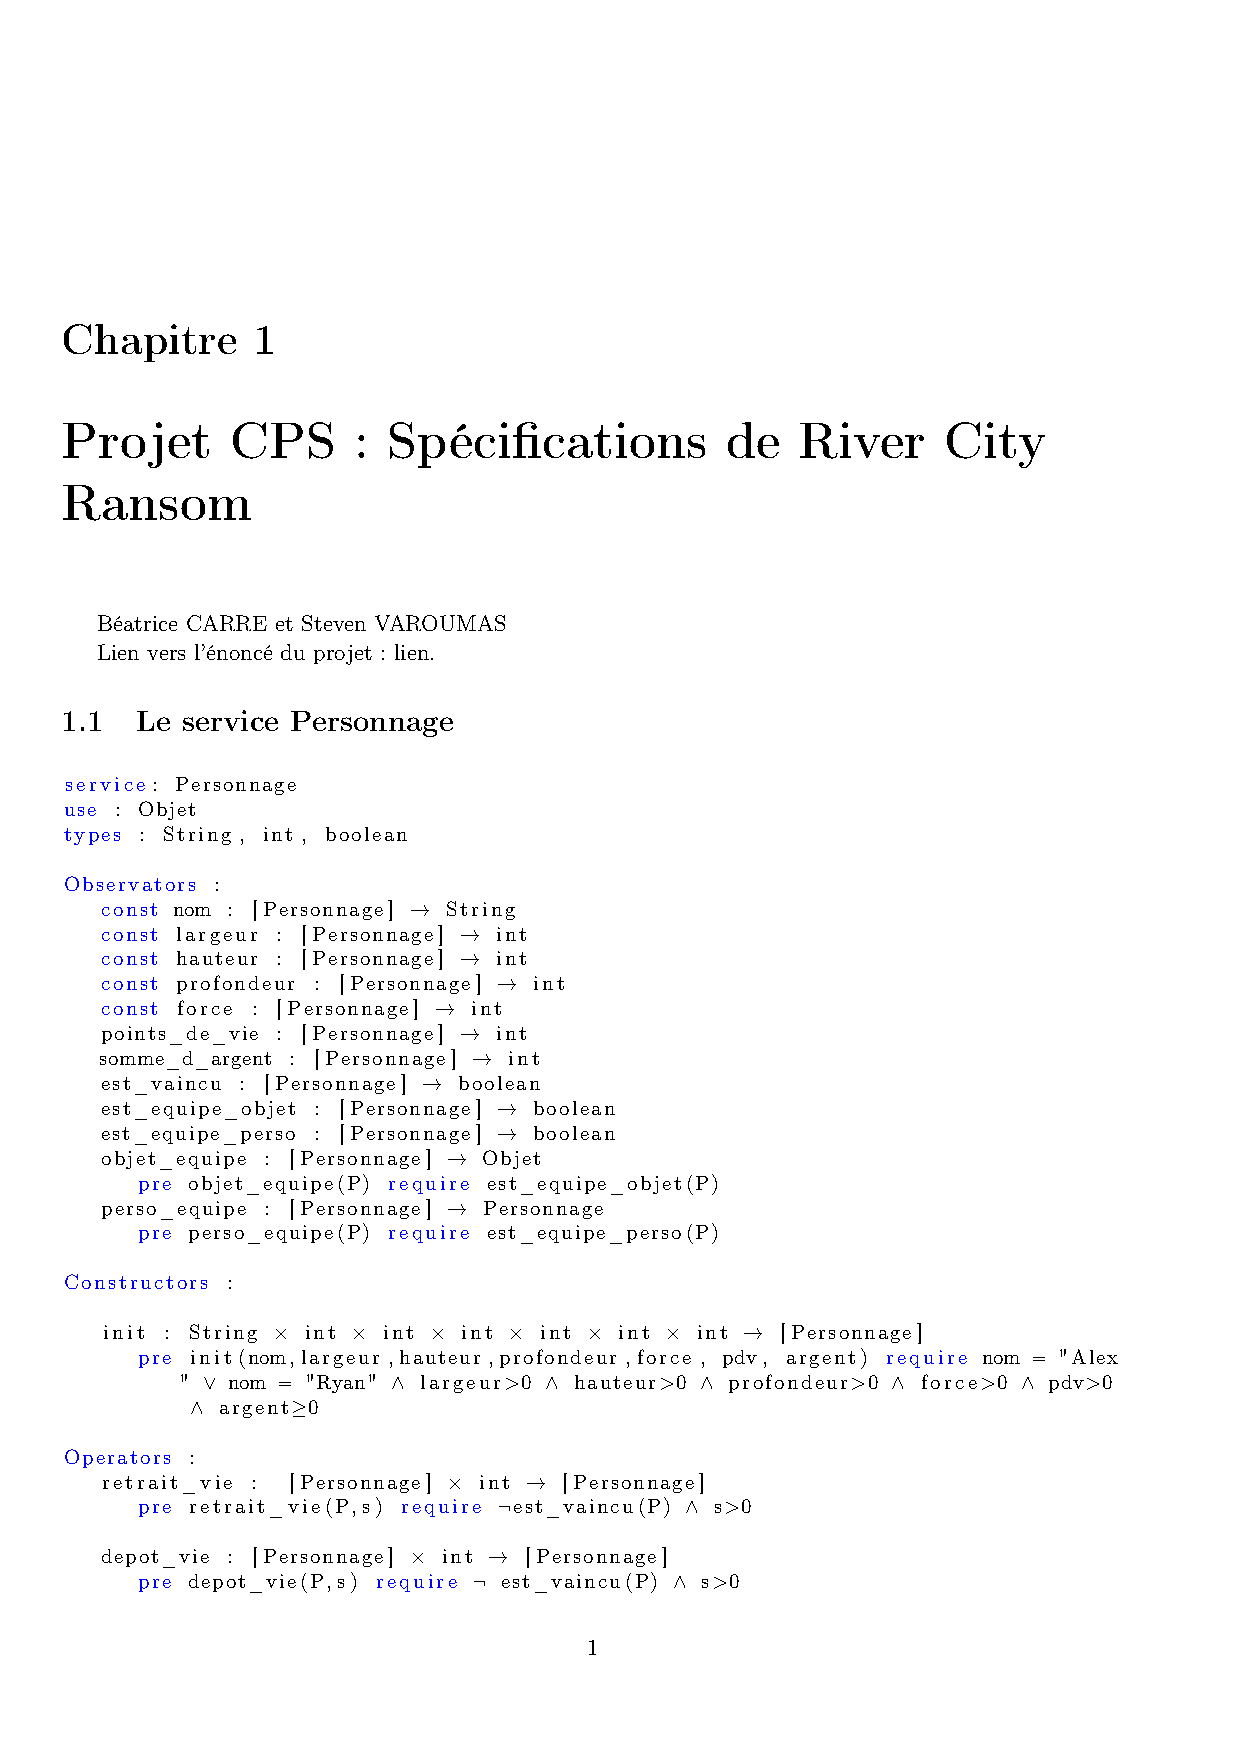
\includepdf[pages={-},pagecommand={},offset=2.cm 1cm]{../Spec/spec.pdf}

\newpage
\pagestyle{empty}
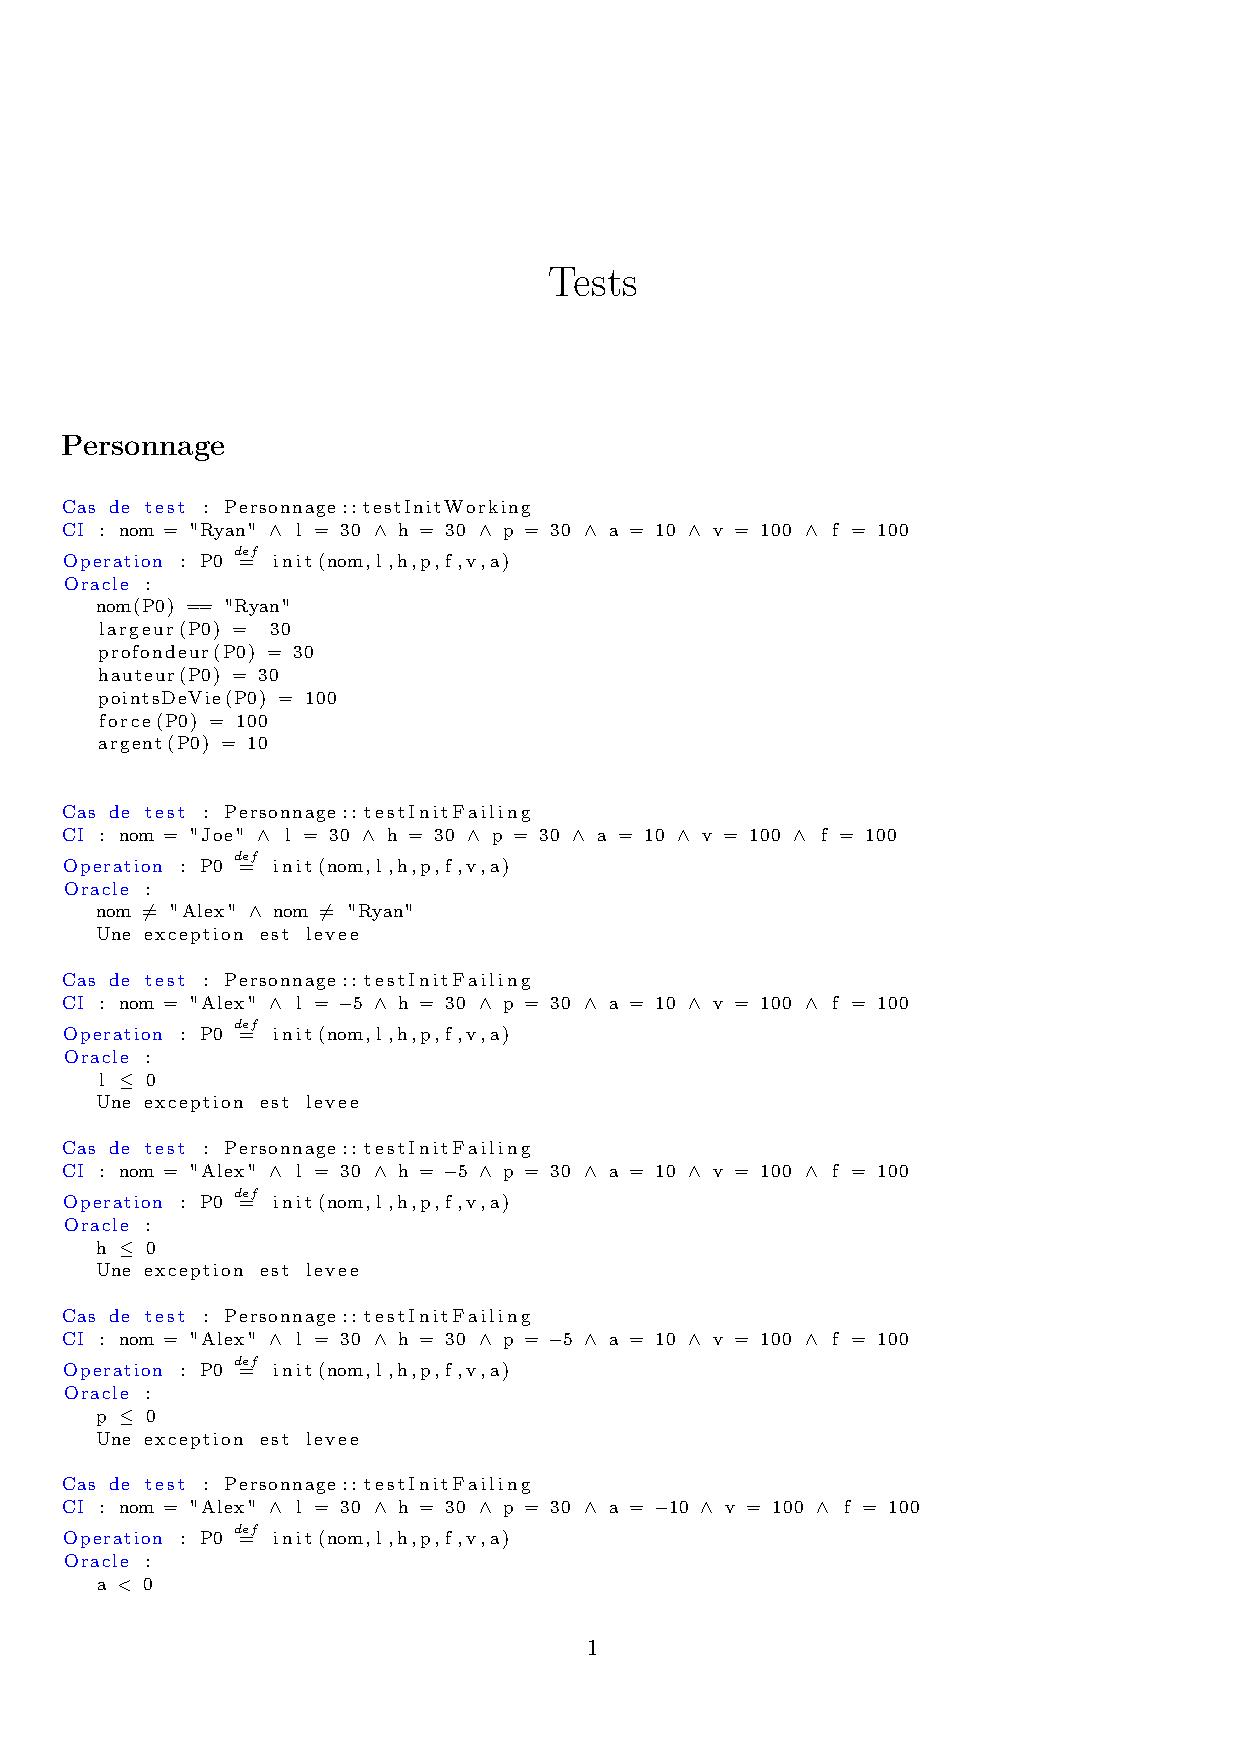
\includepdf[pages={-},pagecommand={},offset=2.cm 1cm]{../Tests/tests.pdf}
\end{document}
